\section{Introduction}
\lettrine[lines=2]{\color{color2}N}{}atural
 selection is a key force in evolution, and a mechanism by
which populations can adapt to external `selection'
pressure. Examples of adaptation abound in the natural
world~\cite{going2016fan}, including for example, classic examples
like lactose tolerance in Northern
Europeans~\cite{bersaglieri2004genetic}, human adaptation to high
altitudes~\cite{yi2010sequencing,simonson2010genetic}, but also drug
resistance in pests~\cite{daborn2001ddt}, HIV~\cite{Feder2016More},
cancer~\cite{gottesman2002mechanisms,zahreddine2013mechanisms},
malarial parasite~\cite{ariey2014molecular,nair2007recurrent}, and
others~\cite{spellberg2008epidemic}. In these examples, understanding
the genetic basis of adaptation can provide valuable information,
underscoring the importance of the problem.


Experimental evolution refers to the study of the evolutionary
processes of a model organism in a controlled
\cite{hegreness2006equivalence,lang2013pervasive,orozco2012adaptation,
  lang2011genetic,barrick2009genome,bollback2007clonal,oz2014strength}
or natural
\cite{maldarelli2013hiv,reid2011new,denef2012situ,winters2012development,
  daniels2013genetic,barrett2008natural,bergland2014genomic}
environment. Recent advances in whole genome sequencing have enabled
us to sequence populations at a reasonable cost, even for large
genomes. Perhaps more important for experimental evolution studies, we
can now evolve and resequence (E\&R) multiple replicates of a population to
obtain \emph{longitudinal time-series data}, in order to investigate
the dynamics of evolution at molecular level.  Although constraints
such as small sizes, limited timescales, and oversimplified
laboratory environments may limit the interpretation of E\&R results,
these studies are increasingly being used to test a wide range of
hypotheses~\cite{kawecki2012experimental} and have been shown to be
more predictive than static data analysis
\cite{boyko2008assessing,desai2008polymorphism,sawyer1992population}.
In particular, longitudinal E\&R data is being used to estimate model
parameters including population
size~\cite{williamson1999using,wang2001pseudo,pollak1983new,waples1989generalized,
  Terhorst2015Multi, jonas2016estimating}, strength of
selection~\cite{mathieson2013estimating,illingworth2011distinguishing,Terhorst2015Multi,
  bollback2008estimation,illingworth2012quantifying,malaspinas2012estimating,
  steinrucken2014novel}, allele age~\cite{malaspinas2012estimating}
recombination rate~\cite{Terhorst2015Multi}, mutation
rate~\cite{Barrick2013Genome, Terhorst2015Multi}, quantitative trait
loci~\cite{baldwin2014power} and for tests of neutrality
hypotheses~\cite{feder2014Identifying,Terhorst2015Multi,burke2010genome,bergland2014genomic}.


While many E\&R study designs are being
used~\cite{Barrick2013Genome,schlotterer2015combining}, we restrict
our attention to the adaptive evolution due to standing variation in fixed size 
populations. This regime has been considered earlier, typically with
\dmel as the model organism of choice, to identify adaptive genes in
longevity and aging ~\cite{burke2010genome,remolina2012genomic} (600
generations), courtship song~\cite{turner2011population} (100
generations), hypoxia tolerance~\cite{zhou2011experimental} (200
generations), adaptation to new laboratory
environments~\cite{orozco2012adaptation,franssen2015patterns} (59
generations), egg size~\cite{jha2015whole} (40 generations), C virus
resistance~\cite{martins2014host} (20 generations), and
dark-fly~\cite{izutsu2015dynamics} (49 generations).


The task of identifying selection signatures can be addressed at
different levels of specificity. At the coarsest level, identification
could simply refer to deciding whether some genomic region (or a gene)
is under selection or not. In the following, we refer to this task as
\emph{detection}. In contrast, the task of \emph{site-identification}
corresponds to the process of finding the favored mutation/allele at
nucleotide level. Finally, \emph{estimation of model parameters}, such
as strength of selection and dominance at the site, can provide a
comprehensive description of the selection process.


In the effort to analyze E\&R selection experiments, many authors
chose to adapt existing tests that were originally used for static
data, pairwise comparisons (two time-points) and single replicates to
perform a null scan.  For instance, Zhu \emph{et
  al.}~\cite{zhou2011experimental} used the ratio of the estimated
population size of case and control populations to compute test
statistic for each genomic region. Burke \emph{et
  al.}~\cite{burke2010genome} applied Fisher exact test to the last
observation of data on case and control populations.  Orozco-terWengel
\emph{et al.}~\cite{orozco2012adaptation} used the
Cochran-Mantel-Haenszel (CMH) test~\cite{agresti2011categorical} to
detect SNPs whose read counts change consistently across all
replicates of two time-point data. Turner \emph{et
  al.}~\cite{turner2011population} proposed the diffStat statistic to
test whether the change in allele frequencies of two populations
deviate from the distribution of change in allele frequencies of two
drifting populations. Bergland \emph{et
  al.}~\cite{bergland2014genomic} calculated $F_{st}$ to populations
throughout time to signify their differentiation from ancestral (two
time-point data) as well as geographically different populations. Jha
\emph{et al.}~\cite{jha2015whole} computed test statistic of
generalized linear-mixed model directly from read counts.


Alternatively, \emph{direct} methods have been developed to analyze
time-series data by taking a likelihood approach, and estimating
population genetics parameters.  Bollback \emph{et
  al.}~\cite{bollback2008estimation} proposed a Hidden Markov Model
(HMM) to estimate the selection coefficient $s$ and population size by
using a diffusion approximation to the Wright Fisher 
process.  Steinr\"{u}cken \emph{et al.}~\cite{steinrucken2014novel}
proposed a general diploid selection model which takes into account of
dominance of the favored allele and approximates likelihood
analytically. Recently, Schraiber \emph{et
  al.}~\cite{schraiber2016bayesian} proposed a Bayesian framework to
estimate parameters using Monte Carlo Markov chain sampling. Mathieson
and McVean~\cite{mathieson2013estimating} adopted HMMs to structured
populations and estimated parameters using an Expectation Maximization
(EM) procedure on discretized allele frequency.  Feder \emph{et
  al.}~\cite{feder2014Identifying} modeled increments in allele
frequency with a Brownian motion process, proposed the Frequency
Increment Test (FIT). More recently, Topa \emph{et
  al.}~\cite{topa2015gaussian} proposed a Gaussian Process (GP) for
modeling single-locus time-series pool-seq data. Terhorst \emph{et
  al.}~\cite{Terhorst2015Multi} extended GP to compute joint
likelihood of multiple loci under null and alternative
hypotheses. Finally, Levy \emph{et al.}~\cite{levy2015quantitative} proposed a
Bayesian model to handle sequencing, amplification and growth noise in
a large population of barcoded lineages.



Among the methods specifically designed for time-series data, many
make assumptions which may not hold in E\&R studies. One common
assumption is that the underlying population size is large, so it is
reasonable to model dynamics of allele frequencies using continuous
state models~\cite{bollback2008estimation, feder2014Identifying,
  Terhorst2015Multi}. Second, many existing methods were originally
designed to process wider time spans seen in ancient DNA studies, an
assumption that does not hold for E\&R
experiments~\cite{steinrucken2014novel,
  schraiber2016bayesian}. Finally, many E\&R analysis tools assume
that allele frequencies in the input data are unbiased
(e.g. ~\cite{bollback2008estimation}), which may not be valid for
shotgun sequencing experiments.

Here, we consider a Hidden Markov Model (HMM), similar to
Williamson~\emph{et al.}~\cite{williamson1999using} and
Bollback~\emph{et al.}'s~\cite{bollback2008estimation} but under a
``small-population-size'' regime. Specifically, we use a discrete
state (frequency) model.  We show that for small population sizes,
discrete models can compute likelihood exactly, which improves
statistical performance, especially for short time-span
experiments. Additionally, we add another level of sampling-noise to
the traditional HMM model, allowing for heterogeneous ascertainment
bias due to uneven coverage among variants. We show that for a wide
range of parameters, \comale\ provides higher power for detecting
selection, estimates model parameters consistently, and localizes
favored allele more accurately compared to the state-of-the-art
methods, while being computationally efficient.

%\lipsum[1-2]
\begin{figure*}
	\centering
	(A)\\
	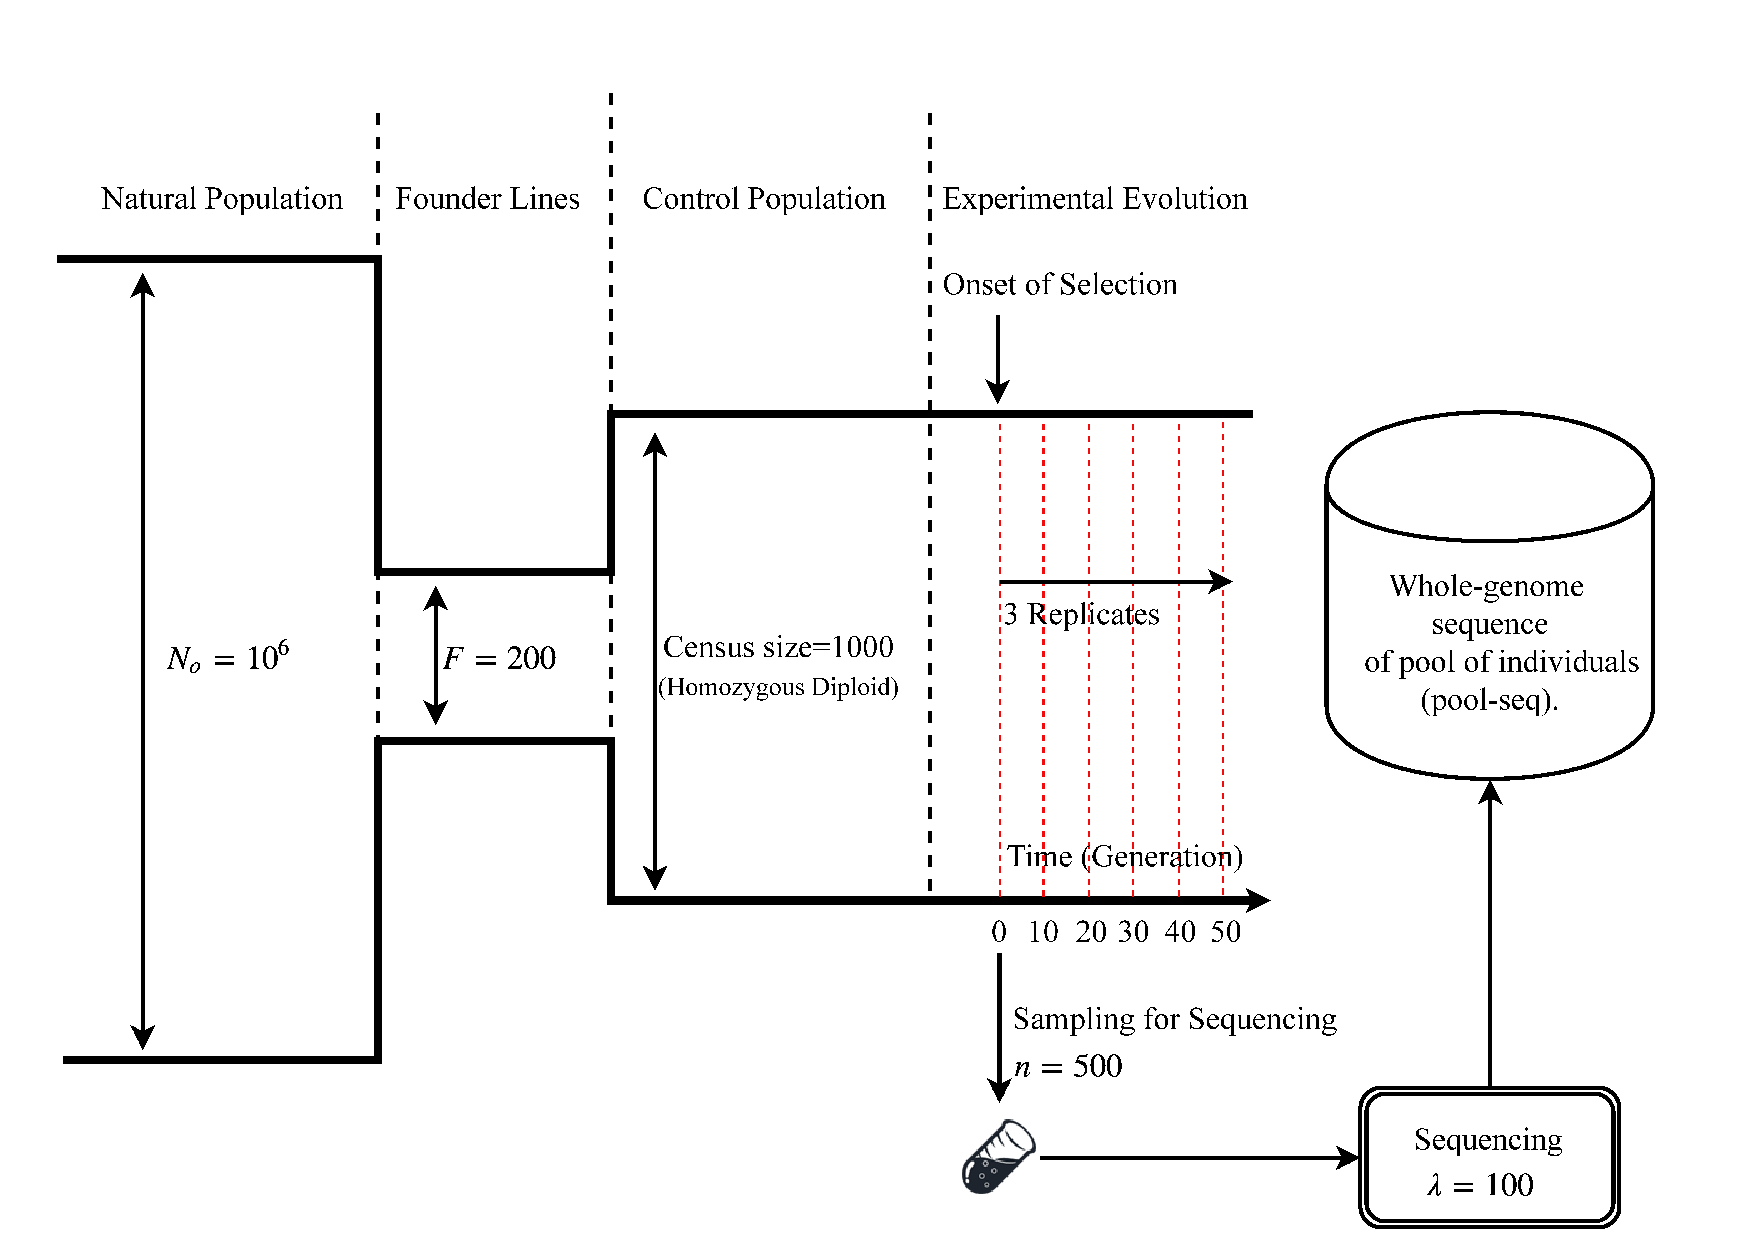
\includegraphics[trim=0in 0in .2in 0.02in , 
	clip,width=0.7\textwidth]{ExperimentalEvolution.pdf}\\
	
	\begin{tabular}{l|l}
		\hline\\
		(B) &(C)\\
		\raisebox{0.1in}{
			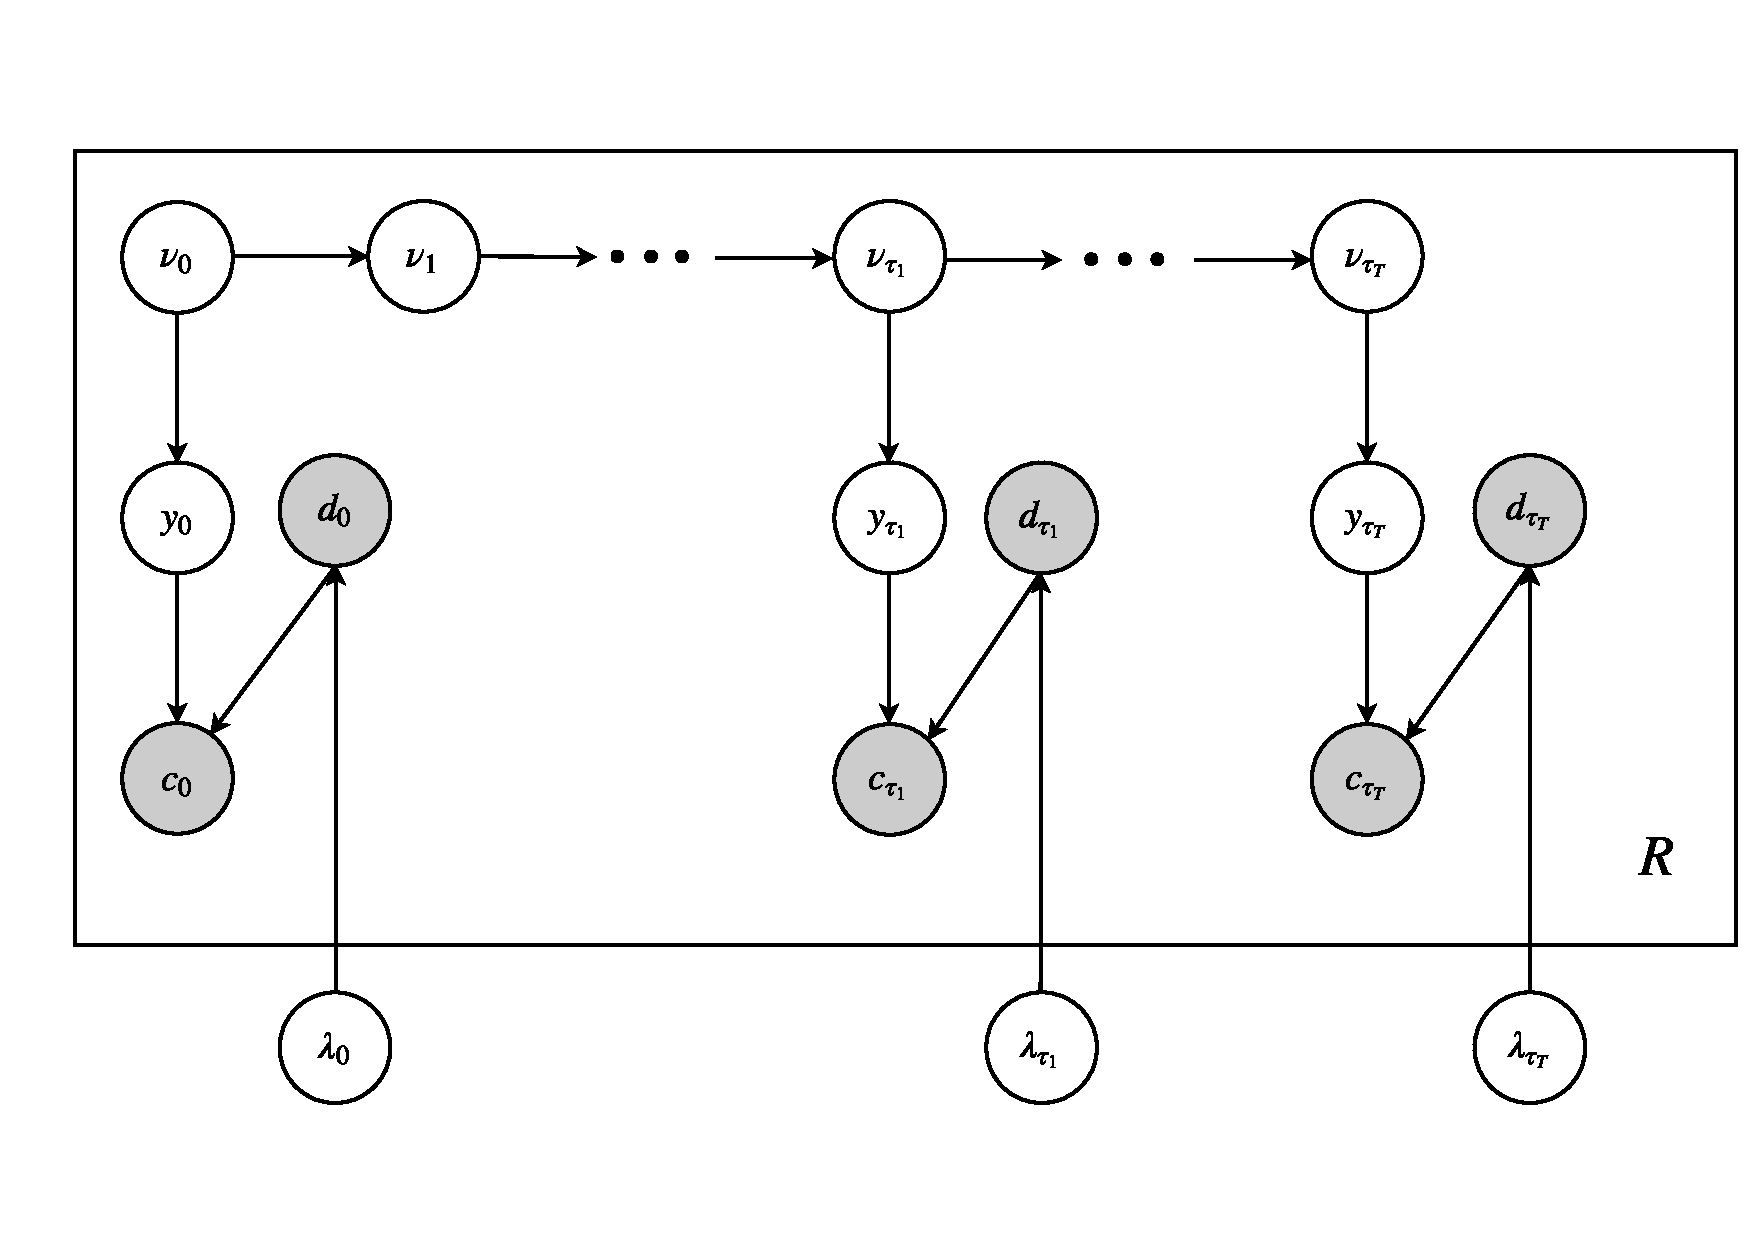
\includegraphics[trim=0in 0.in 0in 
			0.0in,clip,width=0.44\textwidth]{HMMGM.pdf}}
		& 	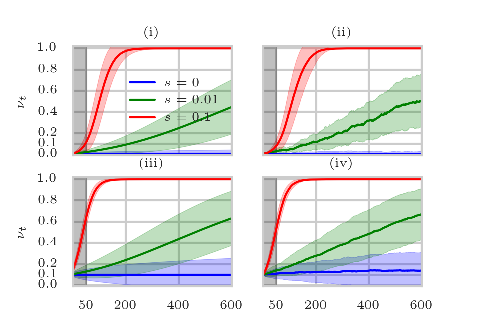
\includegraphics[trim=0in 0.in 0in 
		0.0in,clip,width=0.44\textwidth]{AF.pdf}	
		
	\end{tabular}
	\hspace{-1in}
	\caption{{\bf Evolve and Resequence Selection Experiments on \dmel.}
		(A) Typical configuration in which time-series data is 
		collected for
		\dmel. A small set of founder lines ($F=200$) is selected from a
		large population ($N_o=10^{6}$), and used to create a 
		sub-population
		of isofemale lines. Multiple replicates of the population are
		evolved and resequenced to collect time-series genomic data. For
		sequencing, $n$ individuals are randomly sampled and sequenced 
		with
		coverage $\lambda$.  (B) Graphical model showing dependence of 
		the
		random variables in the single-locus model used to compute 
		\comale\
		statistics. Observed variables, $c$ (derived allele read count) 
		and
		$d$ (total read count) are shaded. The variables $\nu,y,\lambda$
		denote allele frequency, sampled allele frequency, and mean
		sequencing coverage, respectively. (C) Mean and 95\% confidence
		interval of the theoretical (i,iii) and empirical (ii,iv)
		trajectories of the favored allele for hard (i,ii) and soft 
		(iii,iv)
		sweep scenarios and $N=1000$.  The first $50$ generations are 
		shaded
		in gray to represent the sampling span of sampling in short-term
		experiments, illustrating the difficulty in predicting 
		selection at
		early stages of selective sweep.  }
	\label{fig:1}
\end{figure*}
%\lipsum[3-10]